\documentclass[master.tex]{subfiles}

\begin{document}
\section{Monte Carlo Search} 
Monte Carlo Search (MCS) is a family of search techniques that have had much success, particularly within the fields of games, planning and optimization. Generally speaking, MCS is a best-first search strategy that combines random sampling in order to determine an optimal action given a specific domain. In order to describe the ideas of MCS it is useful to be able to describe the domain concretely. To this extent, it is necessary to define the \emph{search domain} \citebay{browne2012survey}, this notation will be used throughout the remainder of this thesis. 

The search domain $\mathbb{S}$ is defined as a 5 - tuple $\mathbb = {S, S_T, A, f, R} $ where: 
\begin{itemize}
\item $S$ - the set of states. 
\item $S_T \subseteq S$ - the terminal states.
\item $A$ - the possible actions.
\item $f : S \times A \rightarrow S$ - the state transition function.
\item $R : S \rightarrow \mathbb{R}^{k} $ - the utility function.
\end{itemize}

Within the domain, an \emph{agent} progresses between states by performing an action.The state $s_0 \in S$ is the unique starting state. At each state $s_i$, an action $a \in A$ is chosen and the agent progresses to the next state $s_{i+1} = f(s_i, a)$. After performing an action, the agent recieves a reward determined by the utility function $R$. Though an agent can obtain a reward for entering any state, rewards are usually only defined for terminal states. These rewards reflect the utility of a certain state and are generally normalized to values between $[0, 1]$. Since it is typically the case that not all actions are valid within a particular state, one can define a function $\alpha : S \rightarrow 2^A$ which given a state $s$ returns all \emph{legal} actions within that state. 

Within the context of search, the idea is to find a sequence of actions $(a_0, a_1, \dots, a_t)$ that leads to a final state $s \in S_t$ such that $R(s)$ is maximized. Such a sequence is thus called an \emph{optimal strategy} or \emph{policy}.  Algorithms such as MCS thus aim to provide approximations for an optimal strategy by estimating the true value of an action through random simulation and then using the actions with the best values in the strategy. The simplest example of MCS called \emph{Flat Monte Carlo} is illustrated in Algorithm \ref{fig:simplemcts}. Given a starting state, the optimal action to play is determined by, for each possible actions, making random playouts until a terminal state is reached, evaluating those states, and  consequently propogating that value back through the tree. The optimal action is then the one which has the largest propogated value.   

\begin{algorithm}
\caption{Flat MCS}
\label{alg:simmcts}
\begin{algorithmic}[1]
\Procedure{FlatMCS}{$s$}
\State $max \gets -\infty$
\For {$a \in \alpha(s)$}
	\State $val \gets R(\textsc{randomRollout}(f(s, a)))$
	\If {$val > max$}
		\State $a_{best} \gets a$
		\State $max \gets val$
	\EndIf
\EndFor
\State \textbf{return} $a_{best}$
\EndProcedure
\Procedure{randomRollout}{$s$}
\State $s_{cur} \gets s$
\While {$s_{cur} \notin S_T$}
	\State $s_{cur} \gets f(s_{cur}, \textsc{getRandom}(\alpha(s_{cur})))$
\EndWhile
\State \textbf{return} $s_{cur}$
\EndProcedure
\end{algorithmic}
\end{algorithm}

\begin{figure}[h!]
\centering

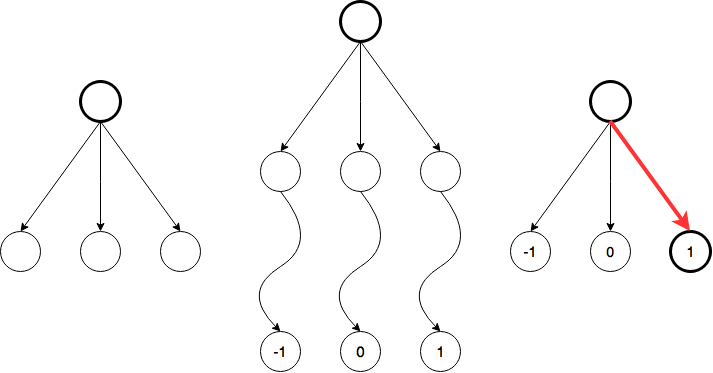
\includegraphics[width=\textwidth]{images/simpleMCTS.png}
\caption{\emph{Example of flat MCS. The right-most action is rated as the best and thus the player chooses to play it.}}
\label{fig:simplemcts}
\end{figure}

The algorithm described in \ref{alg:simmcts} is highly dependant on the random rollouts and thus it is highly likely that the action obtained is not the optimal action. MCS techniques, in general, thus take advantage of repeated simulations in order to obtain more valid approximations to the values of the various actions. 

\subsection{Nested Monte Carlo Search}

Nested Monte Carlo Search (NMCS) is a variant of MCS that uses recursive layers of random simulations in order to determine an optimal move\citebay{cazenave2009nested}. This algorithm (see Algorithm \ref{alg:ncms}) is typically used for 1-player games and thus instead of searching for the best action at a given state, it searches for the whole policy $\pi_{nmcs} = \{s_0, \dots, s_t \}$ \footnote{Here, some liberty is taken in deviating from the definition of the policy $\pi$ as a function. Since NCMS deals with single-player games, it is sufficient to describe $\pi$ as a set of states} where $s_0$ is the initial state and $s_t$ is a possible terminal state. The level $n$ of NMCS defines the depth of recursion that is used in the search. For example a level-0 NMCS algorithm obtains the policy just by performing random rollouts from the initial state until it reaches a terminal state, lines 6 - 10 in the algorithm. NCMS defines utility in terms of policies $R(\pi_{ncms}) \defeq R(s_t)$, i.e, the utility of a policy is the utility of its terminal state. Therefore, NCMS effectively searches to directly find the most optimal terminal state. At higher levels, a level $n$ NCMS algorithm searches for the optimal policy by, for each possible successor state, determining the optimal policy through a level $n-1$ NCMS, lines 14 - 19. The state corresponding to the best optimal policy is chosen as the next state, and the algorithm continues. This idea is illustrated in Figure \ref{fig:nmcs}.
\\
Nested Monte Carlo Search has proven to be an effective algorithm within the domain of single player games such as Morpion, Same Game and Crossword puzzle generation\citebay{cazenave2009nested}. It is because of this success that it is believed that NMCS would be suitable for the problem of first species counterpoint generation.  
 
\begin{figure}[h!]
\centering

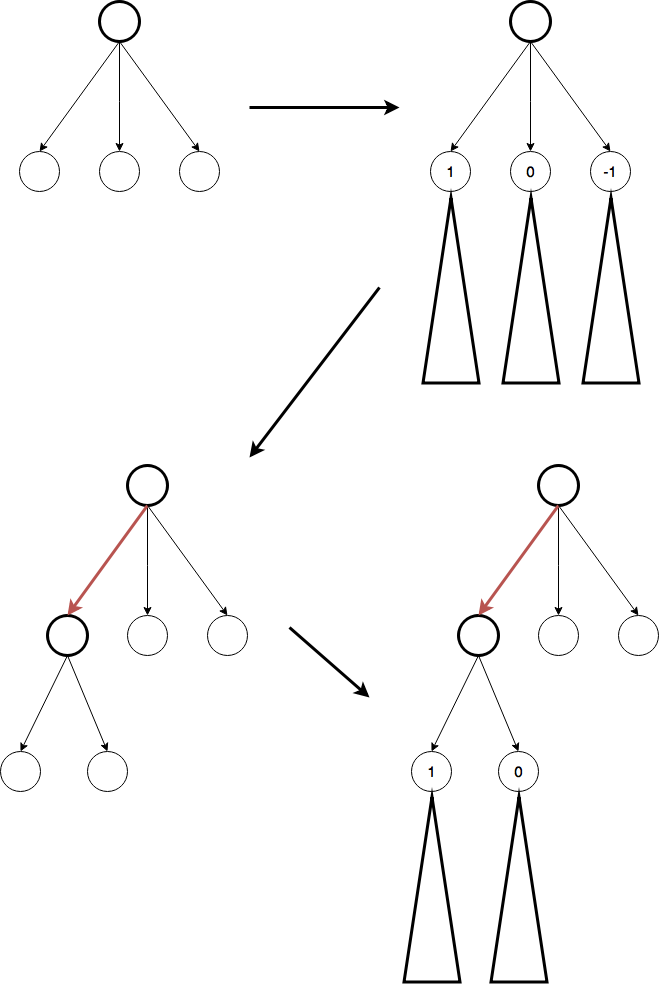
\includegraphics[scale=0.25]{images/NMCS.png}

\caption{\emph{Illustration of the n-level NMCS algorithm. \\The triangles represent an n-1 level NMCS search.}}
\label{fig:nmcs}
\end{figure}

\begin{algorithm}
\caption{Level-n NMCS}
\label{alg:ncms}
\begin{algorithmic}[1]
\Procedure{NCMS}{$n, s$}
\State $ply \gets 0$
\State $\pi \gets \emptyset$
\If {n = 0}
	\State $\pi \gets \{s \}$
	\While {$s \notin S_T$}
		\State $s \gets f(s_{cur}, \textsc{getRandom}(\alpha(s)))$
		\State $\pi.\textsc{add}(s)$
		\State $ply \gets ply + 1$
	\EndWhile
	\State \textbf{return} ($\pi, R(\pi)$)
\Else
	\State $max \gets -\infty$
	\While {$s \notin S_T$}
		\For {$a \in \alpha(s)$}
			\State ($\pi_{temp}, score) \gets NCMS(n - 1,  f(s, a))$
			\If {$score> max$}
				\State $max \gets R(\pi_{temp})$
				\State $\pi.\textsc{add}(s, ply)$
				\State $\pi.\textsc{add}(\pi_{temp}, ply + 1)$
			\EndIf
		\EndFor
		\State $s \gets \pi.\textsc{get}(ply)$
	\EndWhile
	\State \textbf{return} ($\pi, R(\pi)$)
\EndIf
\EndProcedure
\end{algorithmic}
\end{algorithm}

\subsection{Nested Rollout Policy Adaptation} 
Nested Rollout Policy Adaptation (NRPA) is a method based on NMCS created by Rosin \citebay{rosin2011nested}. The algorithm is similar in the sense that it performs nested searches and at level - 0 performs a full playout. The main difference is that, apart from directly traversing the search tree based on the results of previous nested calls, NRPA adapts the rollout policy based on the scores obtained from the nested calls. The idea is that, as search progresses, the policy is updated such that good or promising moves are given increasing probabilities. The algorithm is described in \ref{alg:NRPA}. 

\begin{algorithm}
\caption{Level-n NRPA}
\label{alg:NRPA}
\begin{algorithmic}[1] 
\Procedure{NRPA}{$n, p$}
\If {n = 0} 
	\State $s \gets \text{root()}, ply \gets 0, \pi \gets \emptyset$
	\\
	\While {$s \notin S_T$} 
		 \State $s \gets f(s, \textsc{getRandom}(\alpha (s), p)$
		 \State $\pi.\textsc{add}(s)$
		 \State $ply \gets ply + 1$
	\EndWhile
	\State \textbf{return} ($\pi, R(\pi)$)
\Else
	\State $max \gets -\infty$
	\For {$N$ iterations}
		\State $(\pi_{temp}, score) \gets NRPA(n - 1, p)$
		\\
		\If {$score \geq max$}
			\State $max \gets score$
			\State $\pi \gets \pi_{temp}$
		\EndIf
		\\ 
		\State $p \gets \textsc{adapt}(p, \pi)$
	\EndFor
	\State  \textbf{return} ($\pi, R(\pi)$)
\EndIf
\\
\EndProcedure
\Procedure{adapt}{$p, \pi$}
\State $s \gets  \text{root()}, ply \gets 0, p' \gets p$
\\
\While {$ply < \pi.\textsc{length}()$} 
	\State $s' \gets \pi.\textsc{get}(ply)$
	\State $p'[\textsc{code}(s, s')] \gets p'[\textsc{code}(s, s')]  + \beta$
	\\
	\State $z \gets \sum_{a \in \alpha(s)} \text{exp}(p[code(s, f(s, a))])$
	\\
	\For {$a \in \alpha(s)$}
		\State $p'[code(s, f(s, a))] \gets p'[code(s, f(s, a))] - \frac{\beta}{z}\text{exp}(p[code(s, f(s, a))])$
	\EndFor
	\\
	\State $s \gets s'$
\EndWhile
\State  \textbf{return} $p'$
\EndProcedure
\end{algorithmic}
\end{algorithm}

The algorithm is called with two parameters, $n$ and $p$, the search level and the initial \emph{policy vector}. The policy vector represents the likelihood of an action being selected at a specific state. Therefore, the policy vector must contain a value for each action at each state. These state action pairs are encoded using the function $\textsc{code}(s, s')$, where $s$ represents the current state and $s'$ is the resultant state after applying a specific action.  At level 0, NRPA performs a random playout where each action is chosen proportional to the values in the policy vector, lines 5 - 9. At higher levels, the algorithm searches for $N$ results from $n - 1$ level searches, choosing the best sequence based on its evaluation, lines 12 - 17. The current best sequence is then used to update the values in the policy vector using the $\textsc{adapt}(p, \pi)$ procedure. For all states in the sequence, their weight in the policy vector is increased by a set amount $\beta$. 
\end{document}